\chapter{DDS \& RTPS}\label{SEC:dds}
DDS (Data Distribution Service)\cite{DDS} e RTPS (Real-Time Publish-Subscribe)\cite{RTPS} costituiscono due soluzioni fondamentali nel campo delle comunicazioni distribuite e real-time. Queste tecnologie svolgono un ruolo importante nella la trasmissione di dati tra dispositivi e applicazioni interconnesse, rivestendo particolare importanza in scenari complessi come i sistemi embedded, in IoT e applicazioni ad alte prestazioni come l'HPC (High-Performance Computing). 

\section{DDS}
Data Distribution Service è un protocollo di comunicazione incentrato sullo scambio di dati per sistemi distribuiti. Questo si basa su modello chiamato Data-Centric Publish Subscribe (DCPS) I principali attori che vengono coinvolti sono:
\begin{itemize}
    \item Publisher: responsabile della creazione e configurazione dei DataWriter. Il DataWriter è l'entità responsabile della pubblicazione effettiva dei messaggi. Ciascuno avrà un Topic assegnato sotto il quale vengono pubblicati i messaggi;

    \item Subscriber: responsabile di ricevere i dati pubblicati sotto i topic ai quali si iscrive. Serve uno o più oggetti DataReader, che sono responsabili di comunicare la disponibilità di nuovi dati all'applicazione;

    \item Topic: collega i DataWriter con i DataReader. È univoco all'interno di un dominio DDS;
    
    \item Dominio: utilizzato per collegare tutti i publisher e subscriber appartenenti a una o più domini di appartenenza, che scambiano dati sotto diversi topic. Il DomainParticipant funge da contenitore per altre entità DCPS, e svolge anche la funzione di costruttore di entità Publisher, Subscriber e Topic fornendo anche servizi di QoS;

    \item Partizione: costituisce un isolamento logico di entità all'interno dell'isolamento fisico offerto dal dominio;

\end{itemize}
Inoltre DDS definisce le cosidette Qualità di Servizio (QoS policy) che servono configurare il comportamento di ognuno di questi attori.


\section{RTPS}
Real-Time Publisher Subscribe protocol è un protocollo-middleware utilizzato da DDS per gestire la comunicazione su diversi protocolli di rete come UDP/TCP e Shared Memory. Il suo principale scopo è quello di inviare messaggi real-time, con un approccio best-effort e cercando di massimizzare l'efficienza. E' inoltre progettato per fornire strumenti per la comunicazione unicast e multicast. Le principali entità descritte da RTPS sono:
\begin{itemize}
    \item RTPSWriter: endpoint capace di inviare dati;
    \item RTPSReader: endpoint abilitato alla ricezione dei dati;
\end{itemize}
Ereditato da DDS anche RTPS ha la concezione di Dominio di comunicazione e come questo, le communcazioni a livello di RTPS girano attorno al concetto di Topic prima definito. L'unità di comunicazione è chiamata \textbf{Change} che rappresenta appunto un cambiamento sui dati scritti sotto un certo topic. Ognuno degli attori registra questi \emph{Change} in una struttura dati che funge da cache.
In particolare la sequenza di scambio è:
\begin{enumerate}
    \item il \emph{change} viene aggiunto nella cache del RTPSWriter;
    \item RTPSWriter manda questa \emph{change} a tutti gli RTPSReader che conosce;
    \item quando RTPSReader riceve il messaggio, aggiorna la sua cache con il nuovo \emph{change}.
\end{enumerate}

\begin{figure}[H]
    \centering
    \begin{subfigure}{0.45\linewidth} % Prima immagine
      \centering
      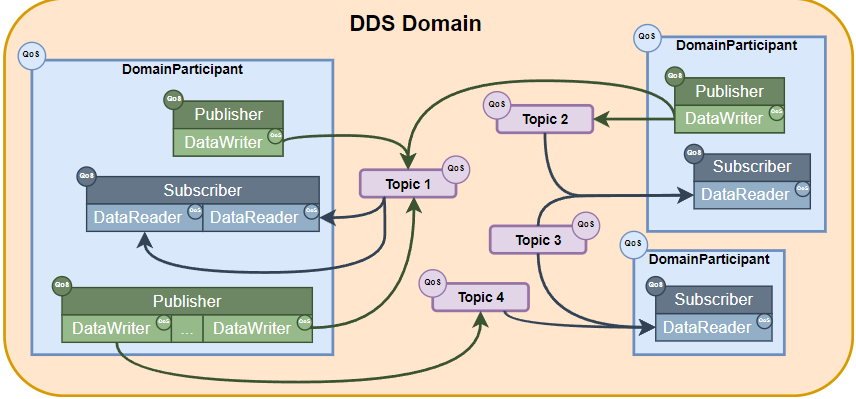
\includegraphics[width=\linewidth]{./img/dds_architecture.png}
      \caption{Schema DDS}
      \label{fig:dds}
    \end{subfigure}
    \begin{subfigure}{0.45\linewidth} % Seconda immagine
      \centering
      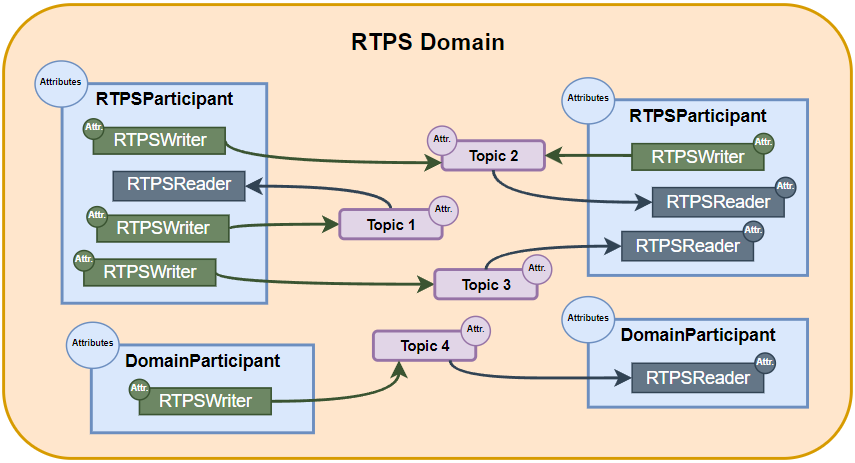
\includegraphics[width=\linewidth]{./img/rtps_architecture.png}
      \caption{Schema RTPS}
      \label{fig:rtps}
    \end{subfigure}
    \caption{Confronto tra architettura DDS e RTPS}
    \label{fig:confrontodds_rtps}
  \end{figure}